\documentclass[ignorenonframetext,]{beamer}
\setbeamertemplate{caption}[numbered]
\setbeamertemplate{caption label separator}{: }
\setbeamercolor{caption name}{fg=normal text.fg}
\beamertemplatenavigationsymbolsempty
\usepackage{lmodern}
\usepackage{amssymb,amsmath}
\usepackage{ifxetex,ifluatex}
\usepackage{fixltx2e} % provides \textsubscript
\ifnum 0\ifxetex 1\fi\ifluatex 1\fi=0 % if pdftex
  \usepackage[T1]{fontenc}
  \usepackage[utf8]{inputenc}
\else % if luatex or xelatex
  \ifxetex
    \usepackage{mathspec}
  \else
    \usepackage{fontspec}
  \fi
  \defaultfontfeatures{Ligatures=TeX,Scale=MatchLowercase}
\fi
% use upquote if available, for straight quotes in verbatim environments
\IfFileExists{upquote.sty}{\usepackage{upquote}}{}
% use microtype if available
\IfFileExists{microtype.sty}{%
\usepackage{microtype}
\UseMicrotypeSet[protrusion]{basicmath} % disable protrusion for tt fonts
}{}
\newif\ifbibliography
\hypersetup{
            pdftitle={DATA 624 - Non-Linear Regression},
            pdfauthor={Omer Ozeren},
            pdfborder={0 0 0},
            breaklinks=true}
\urlstyle{same}  % don't use monospace font for urls
\usepackage{color}
\usepackage{fancyvrb}
\newcommand{\VerbBar}{|}
\newcommand{\VERB}{\Verb[commandchars=\\\{\}]}
\DefineVerbatimEnvironment{Highlighting}{Verbatim}{commandchars=\\\{\}}
% Add ',fontsize=\small' for more characters per line
\usepackage{framed}
\definecolor{shadecolor}{RGB}{248,248,248}
\newenvironment{Shaded}{\begin{snugshade}}{\end{snugshade}}
\newcommand{\KeywordTok}[1]{\textcolor[rgb]{0.13,0.29,0.53}{\textbf{#1}}}
\newcommand{\DataTypeTok}[1]{\textcolor[rgb]{0.13,0.29,0.53}{#1}}
\newcommand{\DecValTok}[1]{\textcolor[rgb]{0.00,0.00,0.81}{#1}}
\newcommand{\BaseNTok}[1]{\textcolor[rgb]{0.00,0.00,0.81}{#1}}
\newcommand{\FloatTok}[1]{\textcolor[rgb]{0.00,0.00,0.81}{#1}}
\newcommand{\ConstantTok}[1]{\textcolor[rgb]{0.00,0.00,0.00}{#1}}
\newcommand{\CharTok}[1]{\textcolor[rgb]{0.31,0.60,0.02}{#1}}
\newcommand{\SpecialCharTok}[1]{\textcolor[rgb]{0.00,0.00,0.00}{#1}}
\newcommand{\StringTok}[1]{\textcolor[rgb]{0.31,0.60,0.02}{#1}}
\newcommand{\VerbatimStringTok}[1]{\textcolor[rgb]{0.31,0.60,0.02}{#1}}
\newcommand{\SpecialStringTok}[1]{\textcolor[rgb]{0.31,0.60,0.02}{#1}}
\newcommand{\ImportTok}[1]{#1}
\newcommand{\CommentTok}[1]{\textcolor[rgb]{0.56,0.35,0.01}{\textit{#1}}}
\newcommand{\DocumentationTok}[1]{\textcolor[rgb]{0.56,0.35,0.01}{\textbf{\textit{#1}}}}
\newcommand{\AnnotationTok}[1]{\textcolor[rgb]{0.56,0.35,0.01}{\textbf{\textit{#1}}}}
\newcommand{\CommentVarTok}[1]{\textcolor[rgb]{0.56,0.35,0.01}{\textbf{\textit{#1}}}}
\newcommand{\OtherTok}[1]{\textcolor[rgb]{0.56,0.35,0.01}{#1}}
\newcommand{\FunctionTok}[1]{\textcolor[rgb]{0.00,0.00,0.00}{#1}}
\newcommand{\VariableTok}[1]{\textcolor[rgb]{0.00,0.00,0.00}{#1}}
\newcommand{\ControlFlowTok}[1]{\textcolor[rgb]{0.13,0.29,0.53}{\textbf{#1}}}
\newcommand{\OperatorTok}[1]{\textcolor[rgb]{0.81,0.36,0.00}{\textbf{#1}}}
\newcommand{\BuiltInTok}[1]{#1}
\newcommand{\ExtensionTok}[1]{#1}
\newcommand{\PreprocessorTok}[1]{\textcolor[rgb]{0.56,0.35,0.01}{\textit{#1}}}
\newcommand{\AttributeTok}[1]{\textcolor[rgb]{0.77,0.63,0.00}{#1}}
\newcommand{\RegionMarkerTok}[1]{#1}
\newcommand{\InformationTok}[1]{\textcolor[rgb]{0.56,0.35,0.01}{\textbf{\textit{#1}}}}
\newcommand{\WarningTok}[1]{\textcolor[rgb]{0.56,0.35,0.01}{\textbf{\textit{#1}}}}
\newcommand{\AlertTok}[1]{\textcolor[rgb]{0.94,0.16,0.16}{#1}}
\newcommand{\ErrorTok}[1]{\textcolor[rgb]{0.64,0.00,0.00}{\textbf{#1}}}
\newcommand{\NormalTok}[1]{#1}

% Prevent slide breaks in the middle of a paragraph:
\widowpenalties 1 10000
\raggedbottom

\AtBeginPart{
  \let\insertpartnumber\relax
  \let\partname\relax
  \frame{\partpage}
}
\AtBeginSection{
  \ifbibliography
  \else
    \let\insertsectionnumber\relax
    \let\sectionname\relax
    \frame{\sectionpage}
  \fi
}
\AtBeginSubsection{
  \let\insertsubsectionnumber\relax
  \let\subsectionname\relax
  \frame{\subsectionpage}
}

\setlength{\parindent}{0pt}
\setlength{\parskip}{6pt plus 2pt minus 1pt}
\setlength{\emergencystretch}{3em}  % prevent overfull lines
\providecommand{\tightlist}{%
  \setlength{\itemsep}{0pt}\setlength{\parskip}{0pt}}
\setcounter{secnumdepth}{0}

\title{DATA 624 - Non-Linear Regression}
\author{Omer Ozeren}
\date{}

\begin{document}
\frame{\titlepage}

\begin{frame}{Linear Regression Models}

\begin{itemize}
\tightlist
\item
  Linear Regression is one of the most basic tools a Data Scientist or
  Analyst can use for analyzing data. It is also used as a prerequiste
  for other advanced regression and machine learning techniques.
\end{itemize}

\begin{block}{Linear Regression model equations can be written either
directly or indirectly in the form:}

\[
\begin{align}
y_i = b_0 +b_1x_{i1} + b_2x_{i2} + ... + b_px_{iP} + \epsilon_i \tag{1}
\end{align}
\]

where

\begin{itemize}
\tightlist
\item
  \(y_i\) represents the numerical response of observation i
\item
  \(b_0\) represents the estimated intercept
\item
  \(b_j\) is the estimated coefficient of the jth predictor
\item
  \(x_{ij}\) is the value of the jth feature of observation i
\item
  P is the number of predictors or explanatory variables
\item
  \(\epsilon_i\) is random error that can't be explained by the model
\end{itemize}

\end{block}

\end{frame}

\begin{frame}{Linear Regression models}

\begin{block}{Goal: to minimize the sum of squared errors (SSE) or a
function of the sum of squared errors}

\begin{block}{Minimize SSE}

OLS - Ordinary Least Squares

PLS - Partial Least Squares

\end{block}

\begin{block}{Minimize a function of the SSE}

Penalized Models

\begin{itemize}
\tightlist
\item
  Ridge Regression
\item
  Lasso
\item
  Elastic Net
\end{itemize}

\begin{block}{Ridge Regression}

\begin{itemize}
\tightlist
\item
  Adds a penalty on the sum of the squared regression parameters and is
  defined by the formula below:
\end{itemize}

\[
\begin{aligned}
SSE_{L_2} = \sum_{i=1}^n (y_i - \hat{y_i})^2 + \lambda \sum_{j=1}^P \beta_j^2
\end{aligned}
\]

\begin{itemize}
\item
  \(L_2\) is for the second-order penalty hence the squared value in the
  parameter estimates.
\item
  What the second term (penalty) does is that the coefficient estimates
  can become large if there is a reduction on the SSE.
\item
  For large \(\lambda\) reduces the estimates near 0. However, the
  parameters never become actually zero and in addition, ridge
  regression does not perform feature selection.
\end{itemize}

\end{block}

\begin{block}{LAsso}

\begin{itemize}
\tightlist
\item
  While ridge regression penalizes the sum of squared coefficnents,
  LASSO penalizes the sum of absolute values that is:
\end{itemize}

\[
\begin{aligned}
SSE_{L_1} = \sum_{i=1}^n (y_i - \hat{y_i})^2 + \lambda \sum_{j=1}^P |{\beta_j}|
\end{aligned}
\]

\begin{itemize}
\item
  Another neat feature is that LASSO may actually make a coefficient = 0
  so therefore it also does feature selection.
\item
  Much like Ridge Regression, we can get the \(\lambda\) value that
  minimizes the MSE as well as extract the coefficients from it. Note
  that if a feature coefficient has just `.' is because LASSO penalized
  that coefficient to be zero and has done feature selection.
\end{itemize}

\end{block}

\begin{block}{Elastic Net}

\begin{itemize}
\item
  LASSO does well when there aren't many parameters and some are already
  close to 0
\item
  Ridge regressions works well if there are many parameters of almost
  the same value.
\item
  LASSO may also take away variables that actually may greatly influence
  the response variable.
\item
  Introducing Elastic Net which combines both and the function is as
  follows:
\end{itemize}

\[
\begin{aligned}
SSE_{E_{net}} = \sum_{i=1}^n (y_i - \hat{y_i})^2 + 
\lambda_1 \sum_{j=1}^P \beta_j^2 + \lambda_2 \sum_{j=1}^P |{\beta_j}|
\end{aligned}
\]

\begin{itemize}
\tightlist
\item
  With this, you get the feature selection power of LASSO and penalties
  of both methods in one.
\end{itemize}

\end{block}

\end{block}

\end{block}

\end{frame}

\begin{frame}{Linear Regression Pros and Cons}

\begin{block}{Advantages:}

\begin{itemize}
\tightlist
\item
  Estimated coefficients allow for interpretation of the relationships
  between predictors
\item
  Coefficient standard errors can be calculated and used to assess the
  statistical significance of each predictor
\end{itemize}

\end{block}

\begin{block}{Disadvantages:}

\begin{itemize}
\tightlist
\item
  They may not be able to adequately capture relationships that are not
  linear
\end{itemize}

\end{block}

\end{frame}

\begin{frame}{Non-Linear Regression}

\begin{block}{Non-linear regression equations take the form:}

\begin{block}{\[y = f(x,\beta) + \varepsilon\]}

Where:

\begin{itemize}
\tightlist
\item
  \(x\) is a vector of \(p\) predictors
\item
  \(\beta\) is a vector of \(k\) parameters
\item
  \(f()\) is a known regression function (that is not linear)
\item
  \(\varepsilon\) is the prediction error term
\end{itemize}

\begin{block}{\emph{Any model equation that cannot be written in the
linear form
\(y_i = b_0 + b_1x_{i1} + b_2x_{i2} + ... + b_Px_{iP} + e_i\) is
non-linear!}}

\end{block}

\end{block}

\end{block}

\end{frame}

\begin{frame}{Non-Linear Regression Pros and Cons}

\begin{block}{Advantages:}

\begin{itemize}
\tightlist
\item
  They can fit almost any functional form and you don't need to know the
  form before training the model
\item
  Can model much more complex relationships between the predictors and
  the outcome than linear models
\end{itemize}

\end{block}

\begin{block}{Disadvantages:}

\begin{itemize}
\tightlist
\item
  Can be computationally expensive
\item
  Some models can be prone to overfitting
\end{itemize}

\end{block}

\end{frame}

\begin{frame}{Non-Linear Regression Model Types}

\begin{block}{Neural Networks (NN)}

Inspired by theories about how the brain works and the
interconnectedness of the neurons in the brain

\end{block}

\begin{block}{Multivariate Regression Splines (MARS)}

Splits each predictor into two groups using a ``hinge'' or
``hockey-stick'' function and models linear relationships to the outcome
for each group separately

\end{block}

\begin{block}{K-Nearest Neighbors (KNN)}

Predicts new samples by finding the closest samples in the training set
predictor space and taking the mean of their response values. K
represents the number of closest samples to consider.

\end{block}

\begin{block}{Support Vector Machines (SVM)}

Robust regression that aims to minimize the effect of outliers with an
approach that uses a subset of the training data points called ``support
vectors'' to predict new values, and counter-intuitively excludes data
points closest to the regression line from the prediction equation.

\end{block}

\end{frame}

\begin{frame}[fragile]{Neural Networks}

\begin{block}{Introduction}

\begin{itemize}
\tightlist
\item
  Neural Network
\end{itemize}

\begin{center}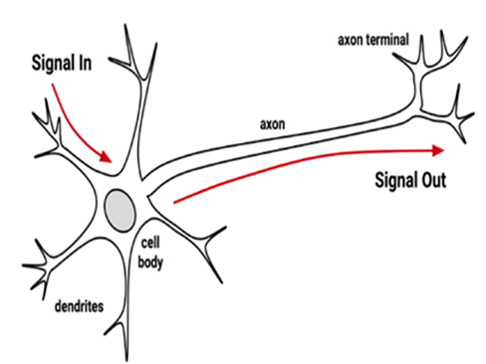
\includegraphics[width=100px]{syn} \end{center}

\begin{center}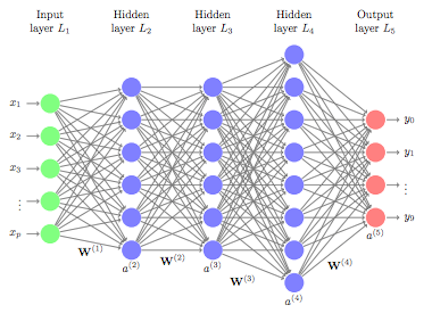
\includegraphics[width=100px]{deep_nn} \end{center}

\begin{itemize}
\tightlist
\item
  Deep Neural Network - Modeled by Neural network of the brain
\item
  Input-Dendrite (Artificial NN Input values)
\item
  Nucleus (Inputs with unique weights and summed together and passed
  threshold in 1 to many hidden layers (neural network 1 layer, deep)
  neural network \textgreater{}1 layers)
\item
  Output - Axon and terminal (Based on about becomes a 0 or 1 with
  Sigmoid function) Transformed by a nonlinear function g().
\end{itemize}

\end{block}

\begin{block}{Computing examples}

\begin{Shaded}
\begin{Highlighting}[]
\CommentTok{# Create Model}
\KeywordTok{library}\NormalTok{(neuralnet)}
\NormalTok{nn<-}\KeywordTok{neuralnet}\NormalTok{(q03_symptoms}\OperatorTok{~}\NormalTok{., }\DataTypeTok{data=}\NormalTok{training, }\DataTypeTok{hidden =}\DecValTok{1}\NormalTok{ , }\DataTypeTok{linear.output=}\OtherTok{FALSE}\NormalTok{, }\DataTypeTok{rep=}\DecValTok{3}\NormalTok{) }
\end{Highlighting}
\end{Shaded}

\begin{itemize}
\tightlist
\item
  Hidden is number of nodes/neuron in a layer, c(2,1) would be 2layers
  with and 1 nodes/neurons
\item
  Can add lifesign= 'full" to get all data points and rep = number of
  repetition times to run model.
\item
  When plotting with Rep can use plot(n, num) to show plot for rep.
\end{itemize}

\end{block}

\begin{block}{Computing examples}

\begin{center}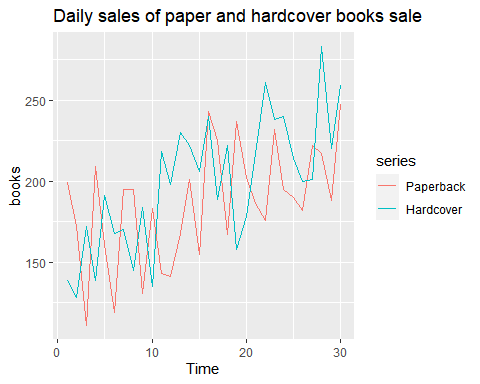
\includegraphics[width=300px]{OmerOzeren_Data624_Presentation_files/figure-beamer/unnamed-chunk-4-1} \end{center}

\begin{verbatim}
## NULL
\end{verbatim}

\begin{verbatim}
##        [,1]       [,2]
## 1 0.9781103 0.01241033
## 2 0.9787063 0.01201374
## 3 0.9787063 0.01201374
## 4 0.9787063 0.01201374
## 6 0.9815269 0.01016525
## 7 0.9787063 0.01201374
\end{verbatim}

\end{block}

\begin{block}{Pros and Cons}

\begin{block}{Pros}

\begin{itemize}
\tightlist
\item
  Robust with noisy data
\item
  Once trained, the predictions are pretty fast.
\item
  Neural networks can be trained with any number of inputs and layers.
\end{itemize}

\end{block}

\begin{block}{Cons}

\begin{itemize}
\tightlist
\item
  Neural networks are black boxes, meaning we cannot know how much each
  independent variable is influencing the dependent variables.
\item
  It is computationally very expensive and time consuming to train with
  traditional CPUs.
\item
  Neural networks depend a lot on training data.
\end{itemize}

\end{block}

\end{block}

\end{frame}

\begin{frame}{Multivariate Adaptive Regression Splines}

\begin{block}{Introduction}

\begin{center}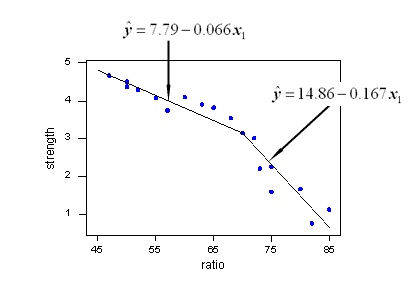
\includegraphics[width=400px]{mars} \end{center}

\begin{itemize}
\tightlist
\item
  Creates 2 contrasted versions to of a predictor
\item
  1 or 2 predictors at a time
\item
  Breaks predictors to 2 groups and models between
\item
  Left-hand - values \textgreater{} 0 than cut point
\item
  Right-hand - values \textless{} 0 than cut point
\end{itemize}

\end{block}

\begin{block}{Pros and Cons}

\begin{block}{Pros}

\begin{itemize}
\tightlist
\item
  MARS models are more flexible than linear regression models.
\item
  MARS models are simple to understand and interpret.
\item
  MARS can handle both continuous and categorical data.
\end{itemize}

\end{block}

\begin{block}{Cons}

\begin{itemize}
\tightlist
\item
  MARS models do not give as good fits as boosted trees, but can be
  built much more quickly and are more interpretable.
\item
  With MARS models, as with any non-parametric regression, parameter
  confidence intervals and other checks on the model cannot be
  calculated directly (unlike linear regression models)
\end{itemize}

\end{block}

\end{block}

\end{frame}

\begin{frame}[fragile]{K-Nearest Neighbors}

\begin{block}{Introduction}

\begin{center}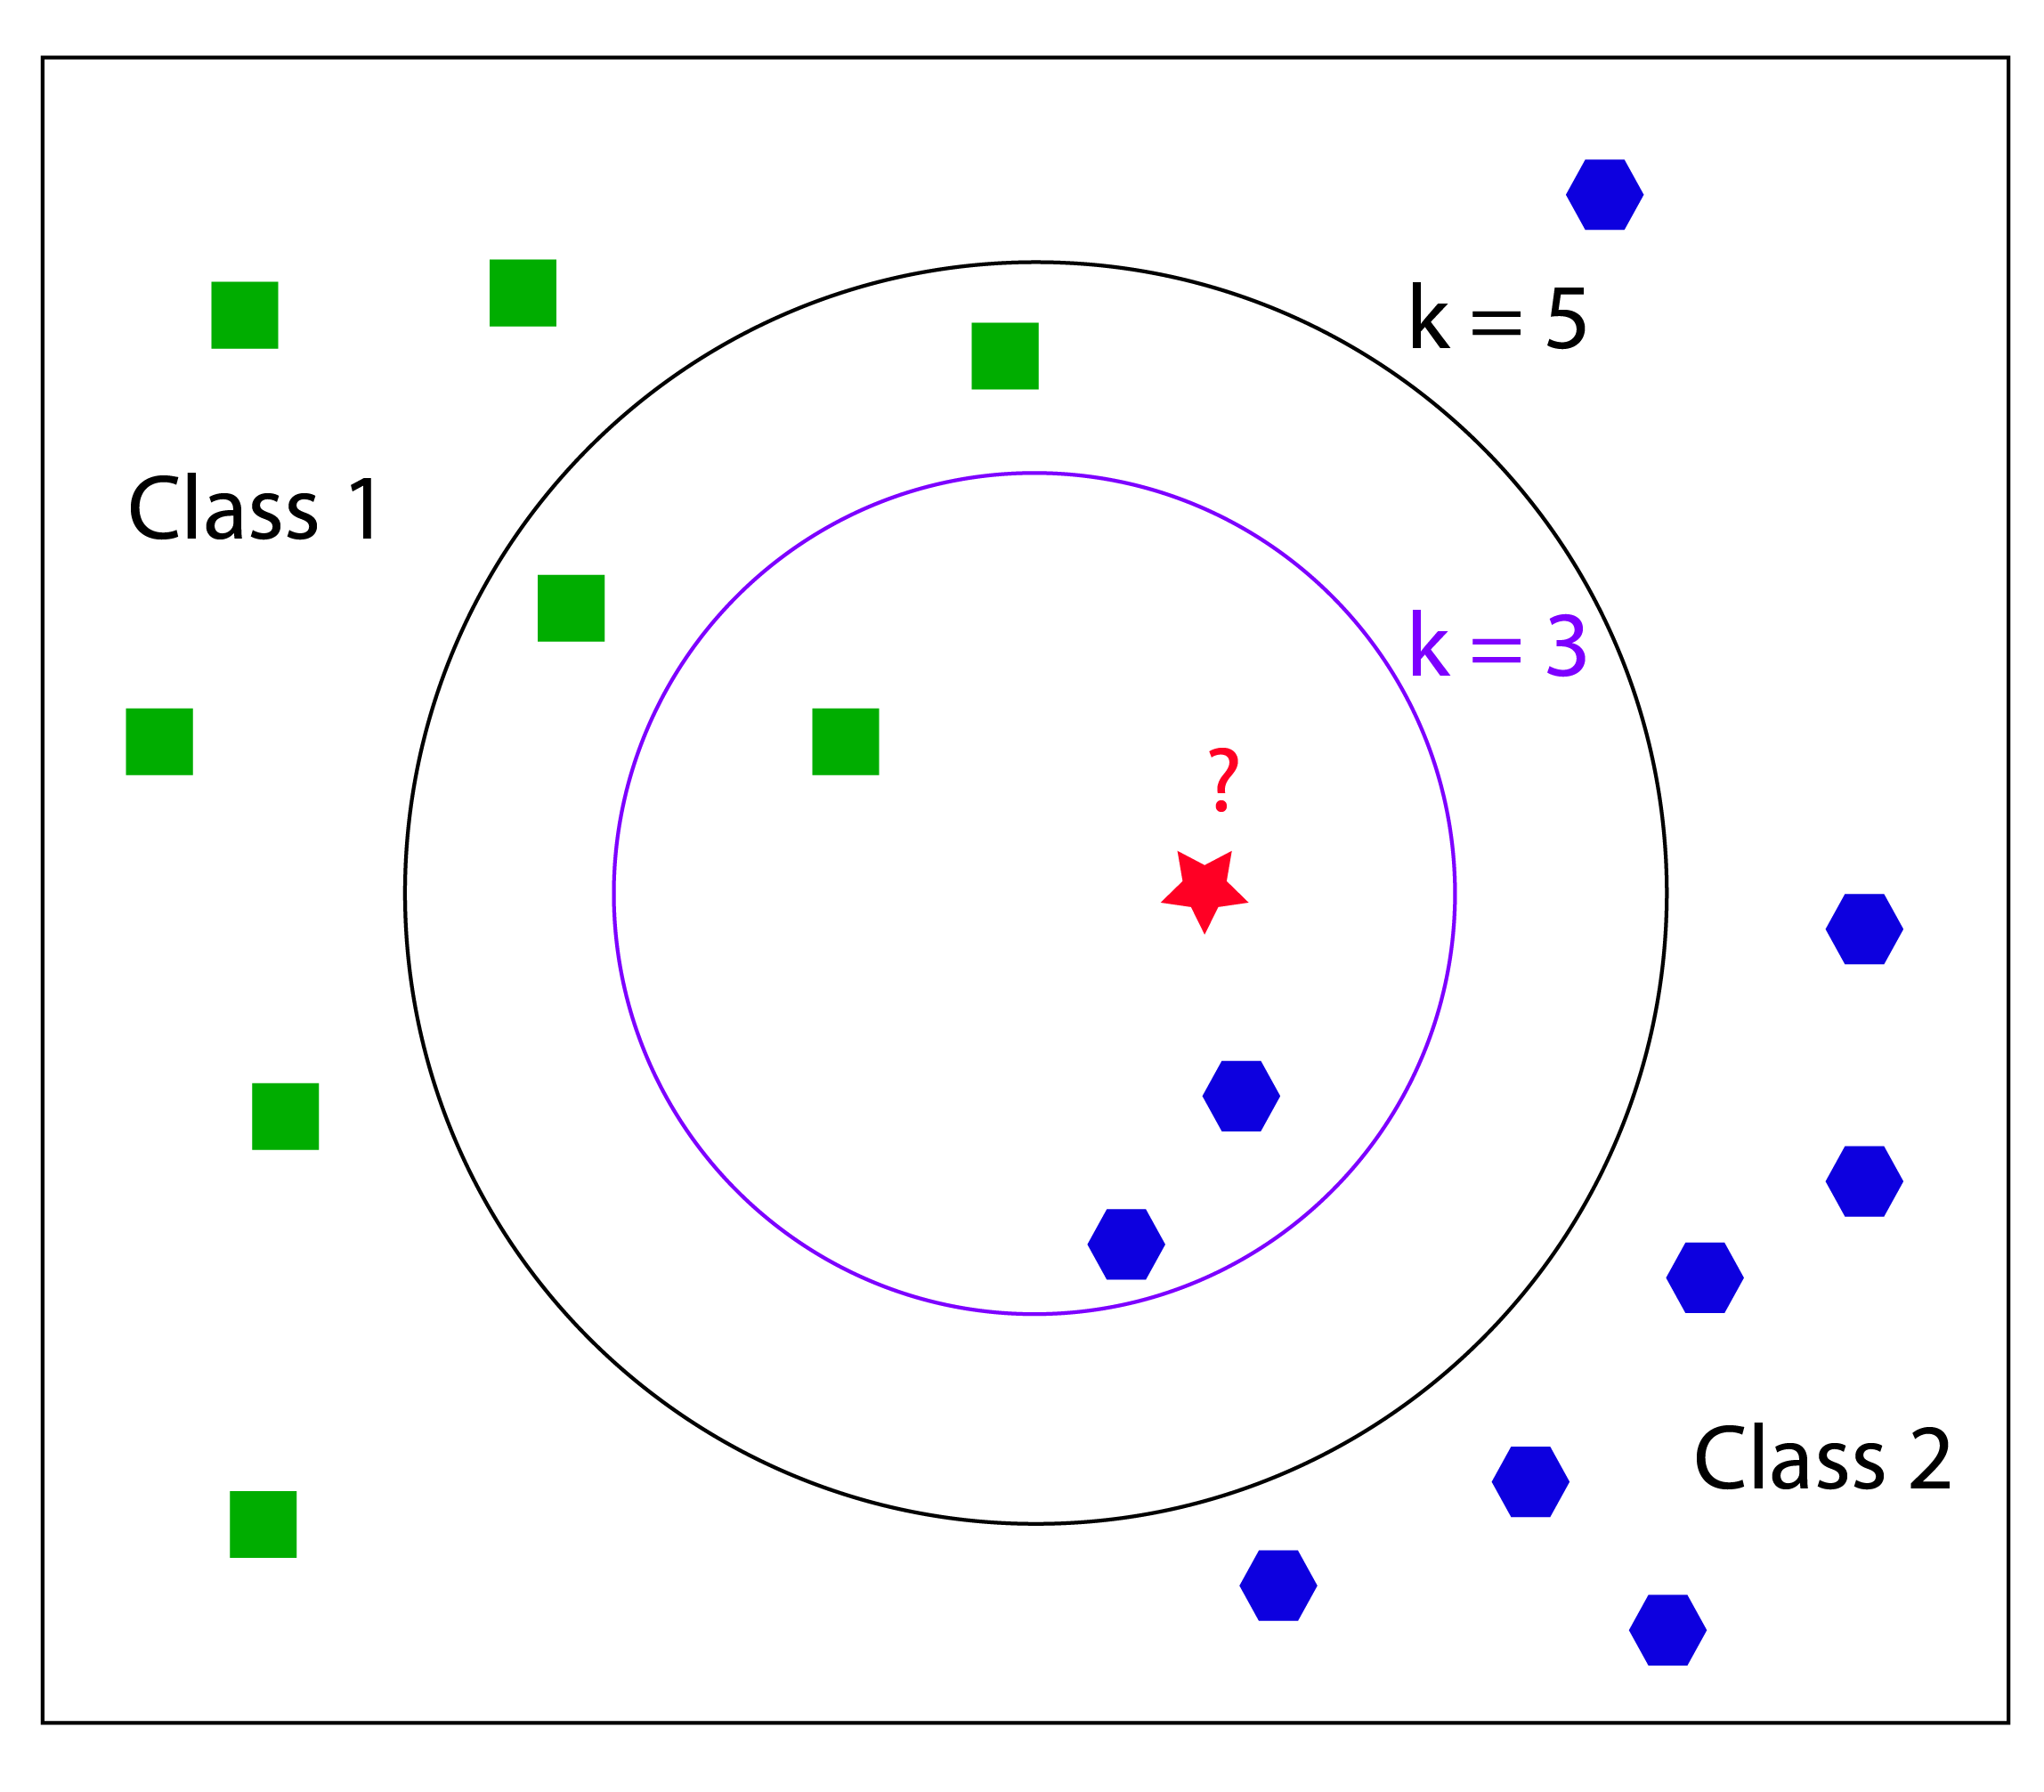
\includegraphics[width=200px]{knn1} \end{center}

\begin{itemize}
\tightlist
\item
  a nonparametric lazy supervised learning method

  \begin{itemize}
  \tightlist
  \item
    does not make any assumptions about data distribution
  \item
    does not require an explicit learning phase for generalization
  \item
    keeps all training examples in memory
  \end{itemize}
\item
  finds k training examples closest to x and returns

  \begin{itemize}
  \tightlist
  \item
    the majority label (through `votes'), in case of classification
  \end{itemize}
\end{itemize}

\end{block}

\begin{block}{Number of Neighbors}

If k = 1, then the new instance is assigned to the class where its
nearest neighbor.

If we give a small (large) k input, it may lead to over-fitting
(under-fitting). To choose a proper k-value, one can count on
cross-validation or bootstrapping.

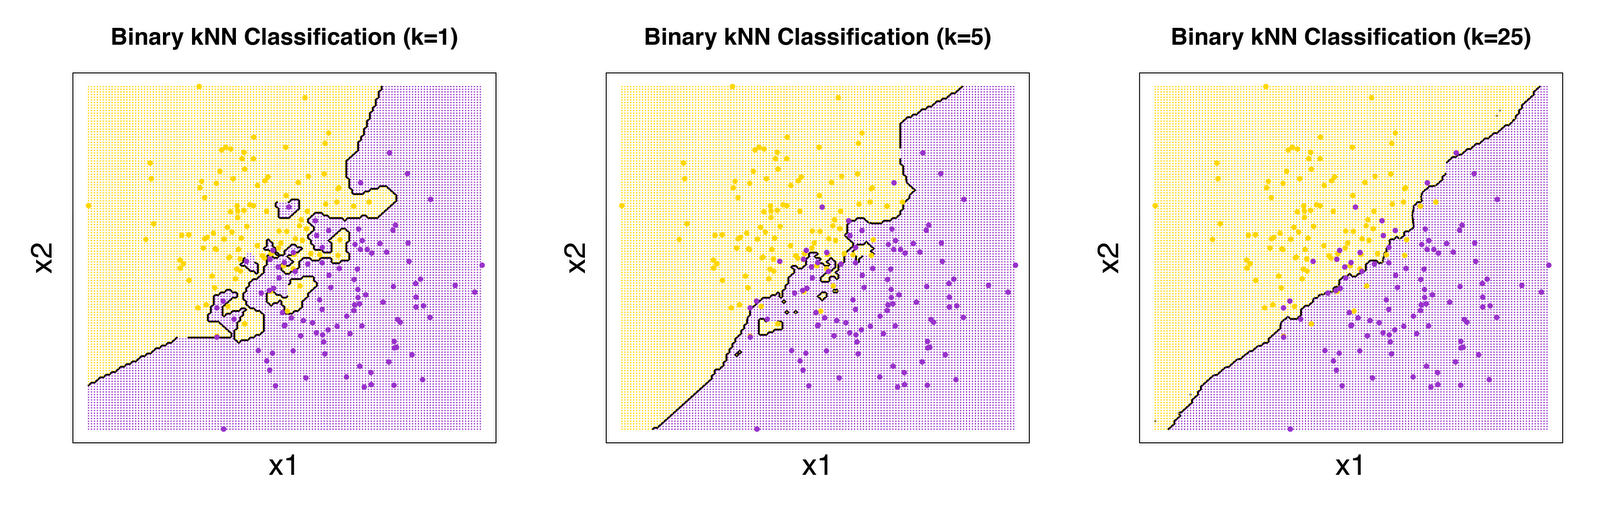
\includegraphics[width=800px]{knn2}

\end{block}

\begin{block}{Similarity/ Distance Metrics}

\begin{itemize}
\tightlist
\item
  knn algorithm performs:

  \begin{itemize}
  \tightlist
  \item
    computation of distance matrix
  \item
    ranking of k most similar objects.
  \end{itemize}
\end{itemize}

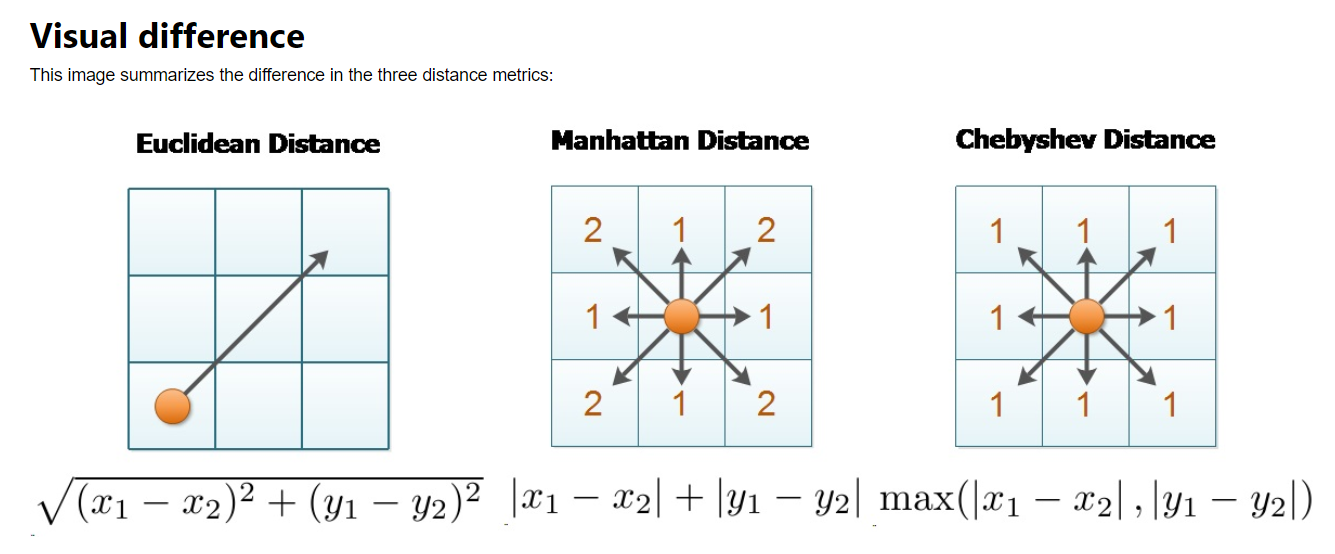
\includegraphics[width=600px]{knn3}

K-Nearest Neighbor Classification of Distance Version method can be
``euclidean'', ``maximum'', ``manhattan'',``canberra'', ``binary'' or
``minkowski''

\begin{Shaded}
\begin{Highlighting}[]
\NormalTok{df <-}\StringTok{ }\KeywordTok{read.table}\NormalTok{(}\StringTok{"C:/Users/OMERO/Documents/GitHub/DATA622/data.txt"}\NormalTok{,}\DataTypeTok{header =}\NormalTok{ T,}\DataTypeTok{sep=}\StringTok{','}\NormalTok{)}
\NormalTok{df}\OperatorTok{$}\NormalTok{label <-}\StringTok{ }\KeywordTok{ifelse}\NormalTok{(df}\OperatorTok{$}\NormalTok{label }\OperatorTok{==}\StringTok{"BLACK"}\NormalTok{,}\DecValTok{1}\NormalTok{,}\DecValTok{0}\NormalTok{)}
\NormalTok{df}\OperatorTok{$}\NormalTok{y <-}\StringTok{ }\KeywordTok{as.numeric}\NormalTok{(df}\OperatorTok{$}\NormalTok{y)}
\NormalTok{df}\OperatorTok{$}\NormalTok{X <-}\StringTok{ }\KeywordTok{as.factor}\NormalTok{(df}\OperatorTok{$}\NormalTok{X)}
\end{Highlighting}
\end{Shaded}

\begin{verbatim}
## [1] 0.5833333
\end{verbatim}

\begin{verbatim}
##       ALGO       AUC       ACC       TPR FPR TNR       FNR
## 1 KNN(K=3) 0.5833333 0.6428571 0.8888889 0.8 0.2 0.1111111
\end{verbatim}

\end{block}

\begin{block}{Advantages \& Disadvantages}

\begin{block}{Pros}

\begin{verbatim}
- cost of the learning process is zero
- nonparametric, K-NN is pretty intuitive and simple
- K-NN has no assumptions
- No Training Step
\end{verbatim}

\end{block}

\begin{block}{Cons}

\begin{verbatim}
- K-NN slow algorithm
- Optimal number of neighbors
- Imbalanced data causes problems
\end{verbatim}

\end{block}

\end{block}

\end{frame}

\begin{frame}[fragile]{Support Vector Machines}

\begin{block}{Introduction}

\begin{center}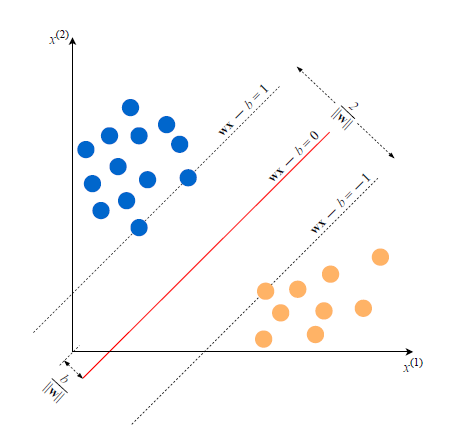
\includegraphics[width=170px]{svm1} \end{center}

\begin{itemize}
\tightlist
\item
  Black box method

  \begin{itemize}
  \tightlist
  \item
    applicable to both supervised regression and classification problems
  \item
    Involves optimally separating (maximal margin) hyperplanes

    \begin{itemize}
    \tightlist
    \item
      in d-dimensional space, a hyperplane is a d-1 dimensional
      separator
    \end{itemize}
  \item
    For non-separable cases, a non-linear mapping transforms the data
    into a kernel-induced feature space F
  \end{itemize}
\end{itemize}

\end{block}

\begin{block}{SVM Applications}

\begin{itemize}
\tightlist
\item
  Bioinformatics

  \begin{itemize}
  \tightlist
  \item
    Protein Structure Prediction
  \item
    Breast Cancer Diagnosis
  \end{itemize}
\item
  Computer vision

  \begin{itemize}
  \tightlist
  \item
    Detecting Steganography in digital images
  \item
    Intrusion Detection
  \item
    Handwriting Recognition
  \end{itemize}
\item
  Computational linguistics
\end{itemize}

\end{block}

\begin{block}{Soft vs.~Hard Margins}

Allow some misclassification by introducing a slack penalty variable
(\(\xi\)). T

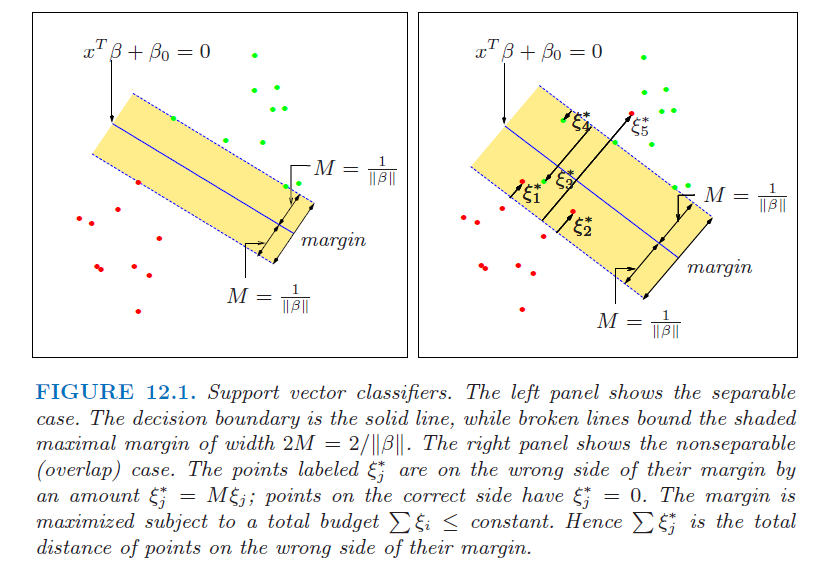
\includegraphics[width=600px]{svm5}

\end{block}

\begin{block}{Cost Penalty}

The slack variable is regulated by hyperparameter cost parameter C. -
when C=0, there is a less complex boundary\\
- when C=inf, more complex boundary, as algorithms cannot afford to
misclassify a single datapoint (overfitting)

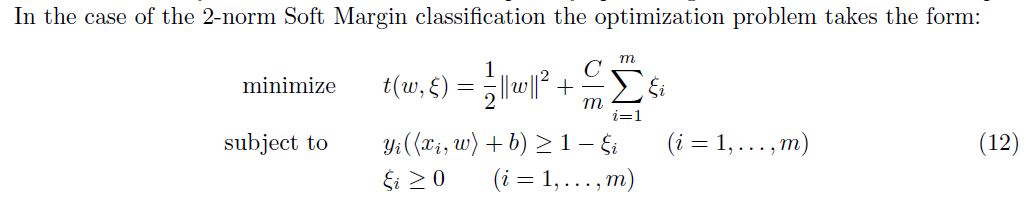
\includegraphics[width=800px]{svm6}

\end{block}

\begin{block}{SVM with High Cost Parameter}

\begin{Shaded}
\begin{Highlighting}[]
\NormalTok{svm.model =}\StringTok{ }\KeywordTok{svm}\NormalTok{(Species }\OperatorTok{~}\StringTok{ }\NormalTok{., }\DataTypeTok{data=}\NormalTok{iris.subset, }\DataTypeTok{type=}\StringTok{'C-classification'}\NormalTok{, }\DataTypeTok{kernel=}\StringTok{'linear'}\NormalTok{, }\DataTypeTok{cost=}\DecValTok{10000}\NormalTok{, }\DataTypeTok{scale=}\OtherTok{FALSE}\NormalTok{)}
\KeywordTok{plot}\NormalTok{(}\DataTypeTok{x=}\NormalTok{iris.subset}\OperatorTok{$}\NormalTok{Sepal.Length,}\DataTypeTok{y=}\NormalTok{iris.subset}\OperatorTok{$}\NormalTok{Sepal.Width, }\DataTypeTok{col=}\NormalTok{iris.subset}\OperatorTok{$}\NormalTok{Species, }\DataTypeTok{pch=}\DecValTok{19}\NormalTok{)}
\KeywordTok{points}\NormalTok{(iris.subset[svm.model}\OperatorTok{$}\NormalTok{index,}\KeywordTok{c}\NormalTok{(}\DecValTok{1}\NormalTok{,}\DecValTok{2}\NormalTok{)],}\DataTypeTok{col=}\StringTok{"blue"}\NormalTok{,}\DataTypeTok{cex=}\DecValTok{2}\NormalTok{)}
\NormalTok{w =}\StringTok{ }\KeywordTok{t}\NormalTok{(svm.model}\OperatorTok{$}\NormalTok{coefs) }\OperatorTok\StringTok{ }\NormalTok{svm.model}\OperatorTok{$}\NormalTok{SV}
\NormalTok{b =}\StringTok{ }\OperatorTok{-}\NormalTok{svm.model}\OperatorTok{$}\NormalTok{rho }\CommentTok{#The negative intercept.}
\KeywordTok{abline}\NormalTok{(}\DataTypeTok{a=}\OperatorTok{-}\NormalTok{b}\OperatorTok{/}\NormalTok{w[}\DecValTok{1}\NormalTok{,}\DecValTok{2}\NormalTok{], }\DataTypeTok{b=}\OperatorTok{-}\NormalTok{w[}\DecValTok{1}\NormalTok{,}\DecValTok{1}\NormalTok{]}\OperatorTok{/}\NormalTok{w[}\DecValTok{1}\NormalTok{,}\DecValTok{2}\NormalTok{], }\DataTypeTok{col=}\StringTok{"red"}\NormalTok{, }\DataTypeTok{lty=}\DecValTok{5}\NormalTok{)}
\end{Highlighting}
\end{Shaded}

\end{block}

\end{frame}

\begin{frame}{Support Vector Machines}

\begin{block}{Kernel Trick}

All kernel functions take two feature vectors as parameters and return
the scalar dot (inner) product of the vectors. Have property of symmetry
and is positive semi-definite.

By performing convex quadratic optimization, we may rewrite the
algorithm so that it is independent of transforming function \(\phi\)

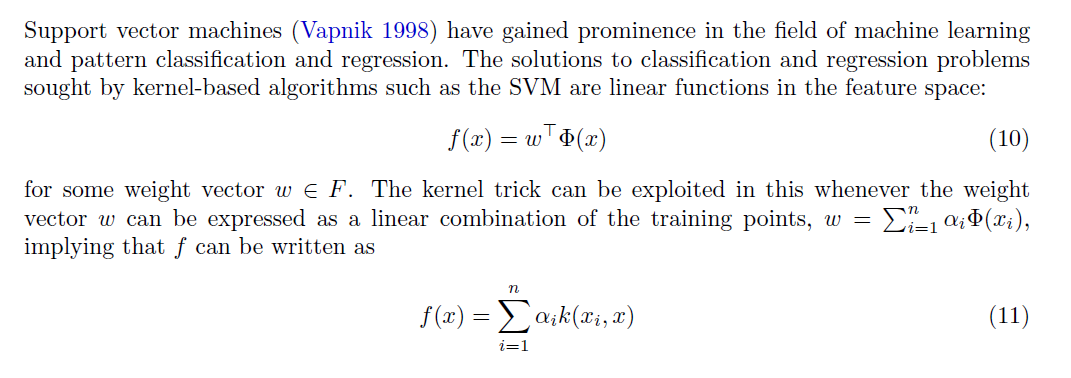
\includegraphics[width=800px]{svm7}

\end{block}

\end{frame}

\begin{frame}[fragile]{Support Vector Machines}

\begin{block}{Model Tuning (Cost \& Gamma)}

\begin{itemize}
\item
  One can tune hyperparameters (cost and gamma) using tune.svm() in
  e1071 and train() in caret
\item
  For the gamma argument,

  \begin{itemize}
  \tightlist
  \item
    the default value is equal to (1/data dimension), and
  \item
    it controls the shape of the separating hyperplane.
  \item
    Increasing the gamma argument usually increases the number of
    support vectors.
  \end{itemize}
\end{itemize}

\begin{Shaded}
\begin{Highlighting}[]
\NormalTok{tuned =}\StringTok{ }\KeywordTok{tune.svm}\NormalTok{(Species}\OperatorTok{~}\NormalTok{., }\DataTypeTok{data =}\NormalTok{ iris.subset, }\DataTypeTok{gamma =} \DecValTok{10}\OperatorTok{^}\NormalTok{(}\OperatorTok{-}\DecValTok{6}\OperatorTok{:-}\DecValTok{1}\NormalTok{),}\DataTypeTok{cost =} \DecValTok{10}\OperatorTok{^}\NormalTok{(}\DecValTok{0}\OperatorTok{:}\DecValTok{2}\NormalTok{))}
\NormalTok{model.tuned =}\StringTok{ }\KeywordTok{svm}\NormalTok{(Species}\OperatorTok{~}\NormalTok{., }\DataTypeTok{data =}\NormalTok{ iris.subset, }\DataTypeTok{gamma =}\NormalTok{ tuned}\OperatorTok{$}\NormalTok{best.parameters}\OperatorTok{$}\NormalTok{gamma, }\DataTypeTok{cost =}\NormalTok{ tuned}\OperatorTok{$}\NormalTok{best.parameters}\OperatorTok{$}\NormalTok{cost)}
\end{Highlighting}
\end{Shaded}

\end{block}

\end{frame}

\begin{frame}{Support Vector Machines}

\begin{block}{Advantages \& Disadvantages}

\begin{itemize}
\tightlist
\item
  Strengths

  \begin{itemize}
  \tightlist
  \item
    effective in high dimensional spaces (dim \textgreater{} N)
  \item
    effective in cases where the number of dimensions is greater than
    the number of samples.
  \item
    It works really well with a clear margin of separation
  \item
    It uses a subset of training points in the decision function (called
    support vectors), so it is also memory efficient.
  \item
    It is effective in high dimensional spaces.
  \end{itemize}
\item
  Drawbacks

  \begin{itemize}
  \tightlist
  \item
    It fails to perform well, when we have large data set because the
    required training time is higher
  \item
    SVM doesn't directly provide probability estimates
  \item
    It fails to perform, when the data set has more noise
  \end{itemize}
\end{itemize}

\end{block}

\end{frame}

\end{document}
